\documentclass[12pt,a4paper,oneside]{ctexart}
\title{\textbf{Practice4 Report}}
\author{Name:Xu Ziyang 22320607}
\date{2023/11/3 YY/MM/DD}
\usepackage{graphicx}
\usepackage{float}
\usepackage{color}
\usepackage{amsmath}
\begin{document}
    \maketitle
    \newpage
    \begin{abstract}
        This Practice work is mainly about how to transform a linear system between state-space form and diffrencial equation form.
        I used subsystem to show all models. The transfer function is used to check if I was right.Here is the overview of systems:
        \begin{figure}[H]
            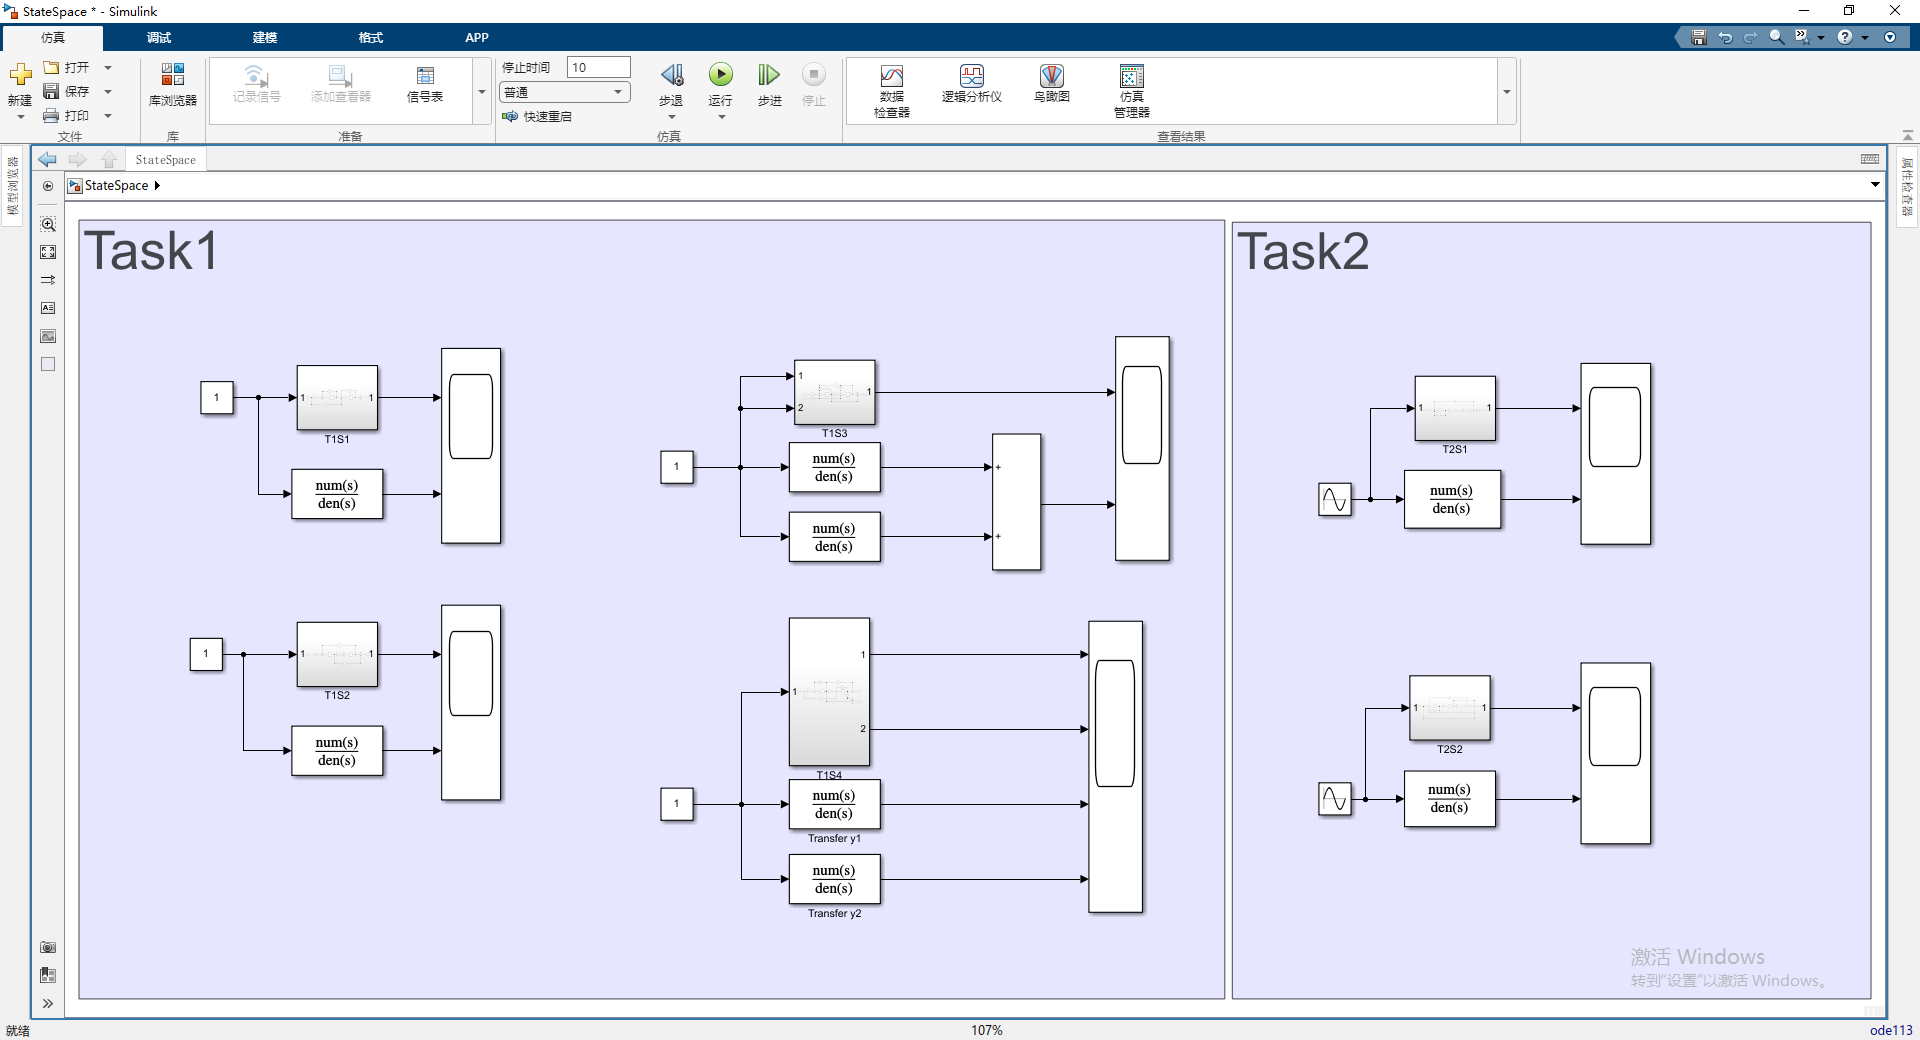
\includegraphics[width = 0.9\linewidth]{../screenshots/MOverView}
            \caption{Overview of systems}
        \end{figure}
    \end{abstract}

    \section{Constructing Systems}
    \textbf{Here shows the Detail of subsystem:}
    \subsection{Task1}
    \newpage
    \begin{figure}[H]
        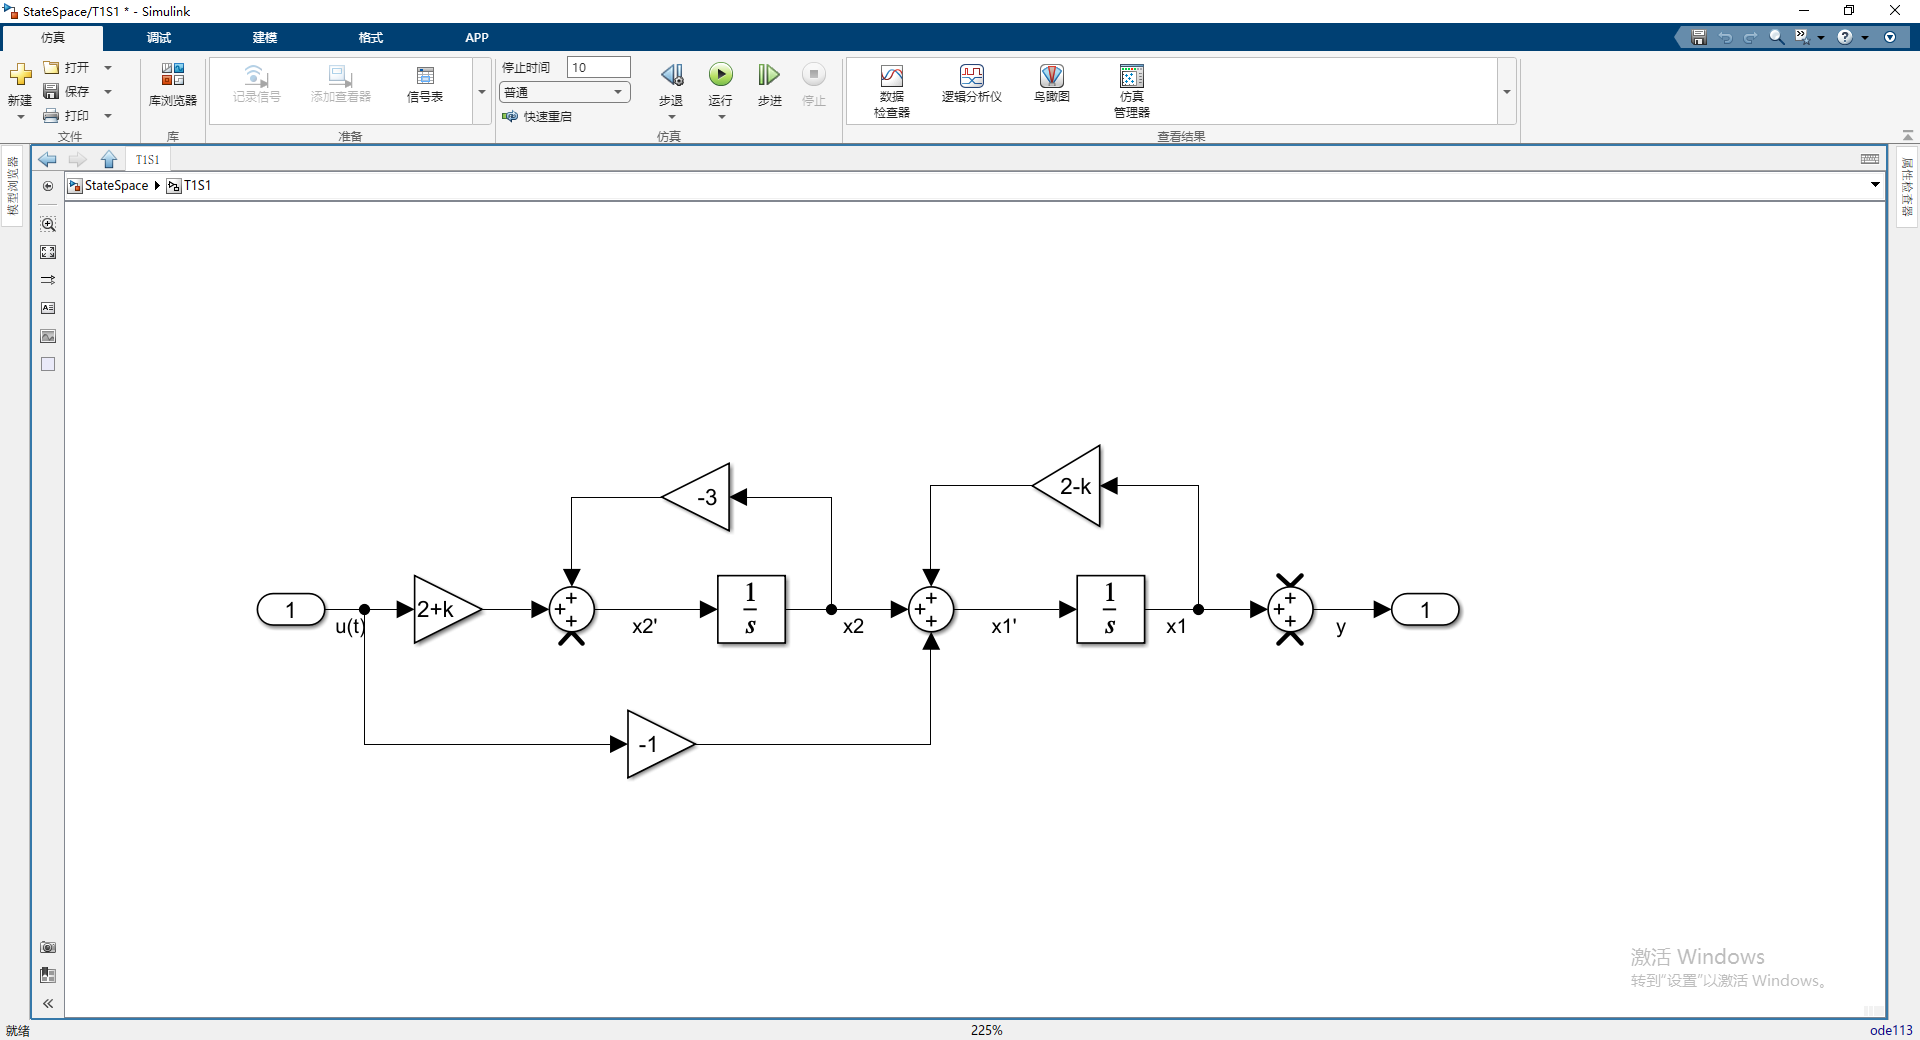
\includegraphics[height = 0.35\textheight]{../screenshots/MT1S1.PNG}
        \caption{System1}
        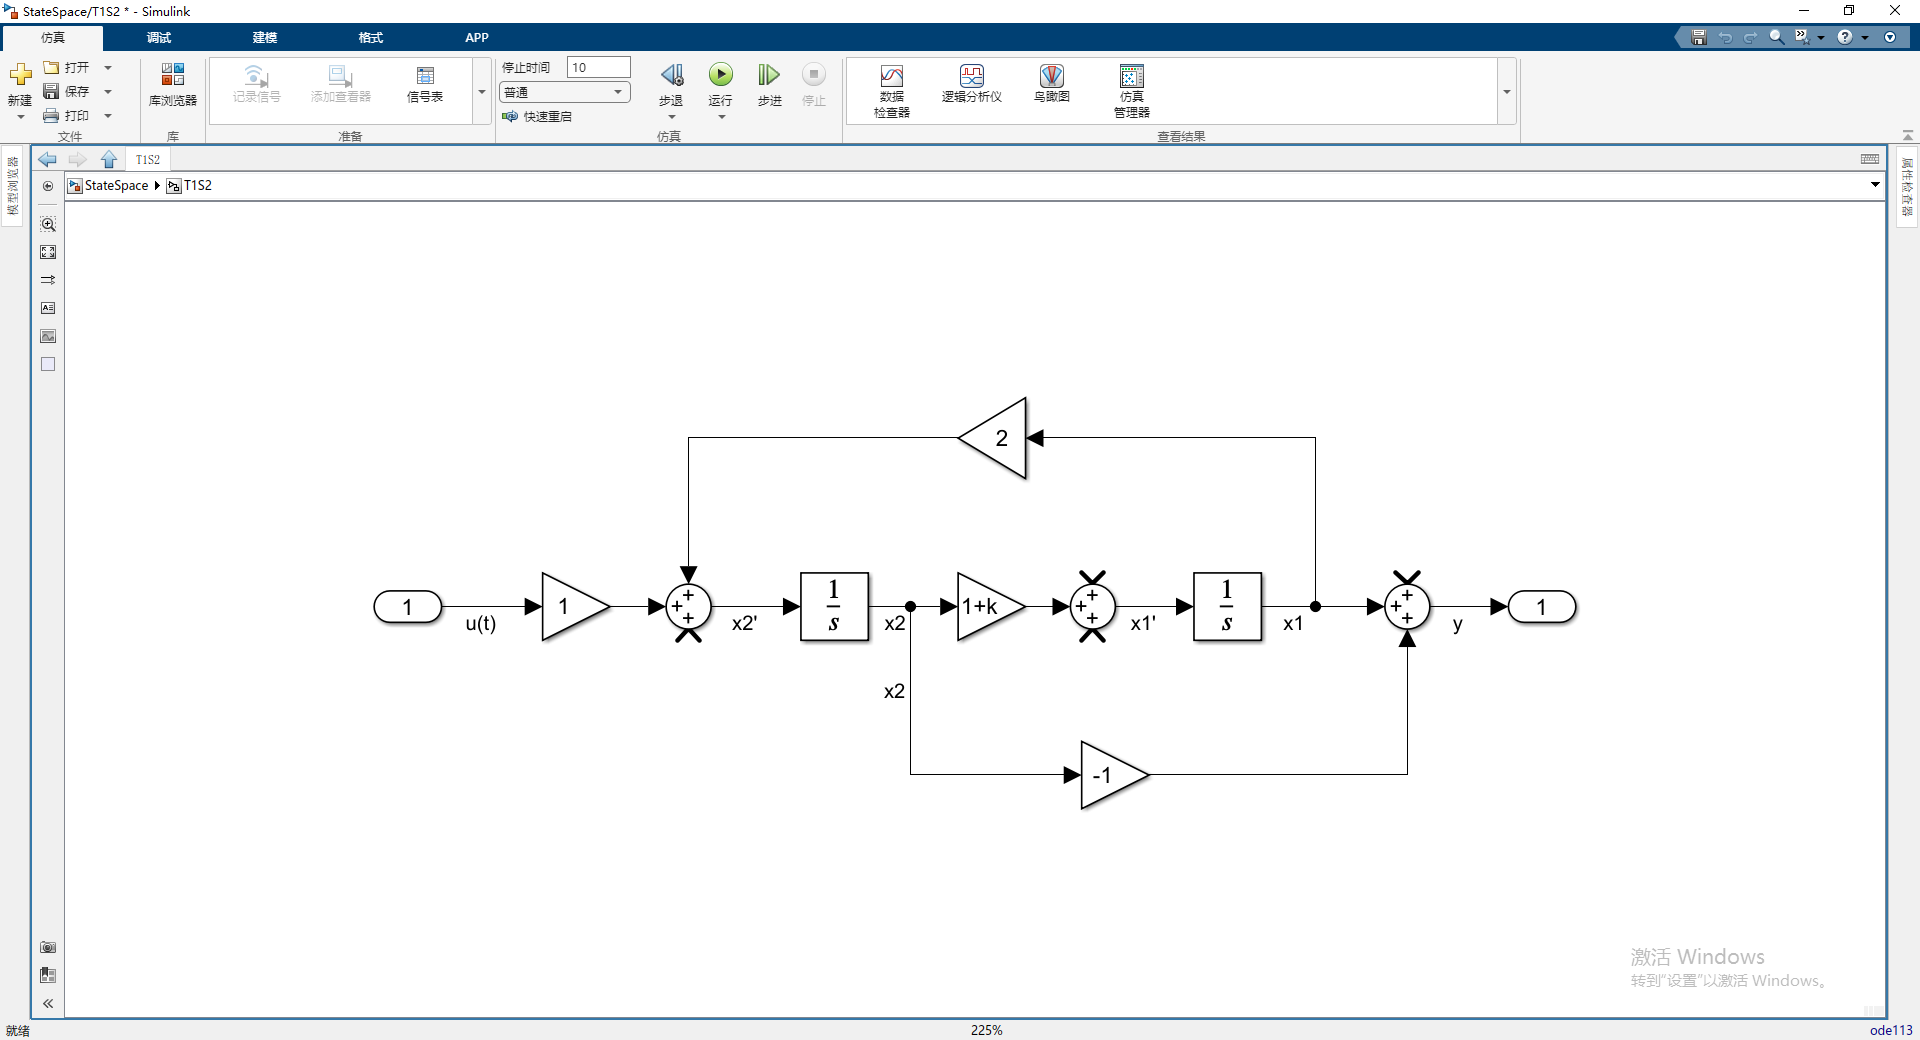
\includegraphics[height = 0.35\textheight]{../screenshots/MT1S2.PNG}
        \caption{System2}
    \end{figure}
    \newpage
    \begin{figure}[H]
        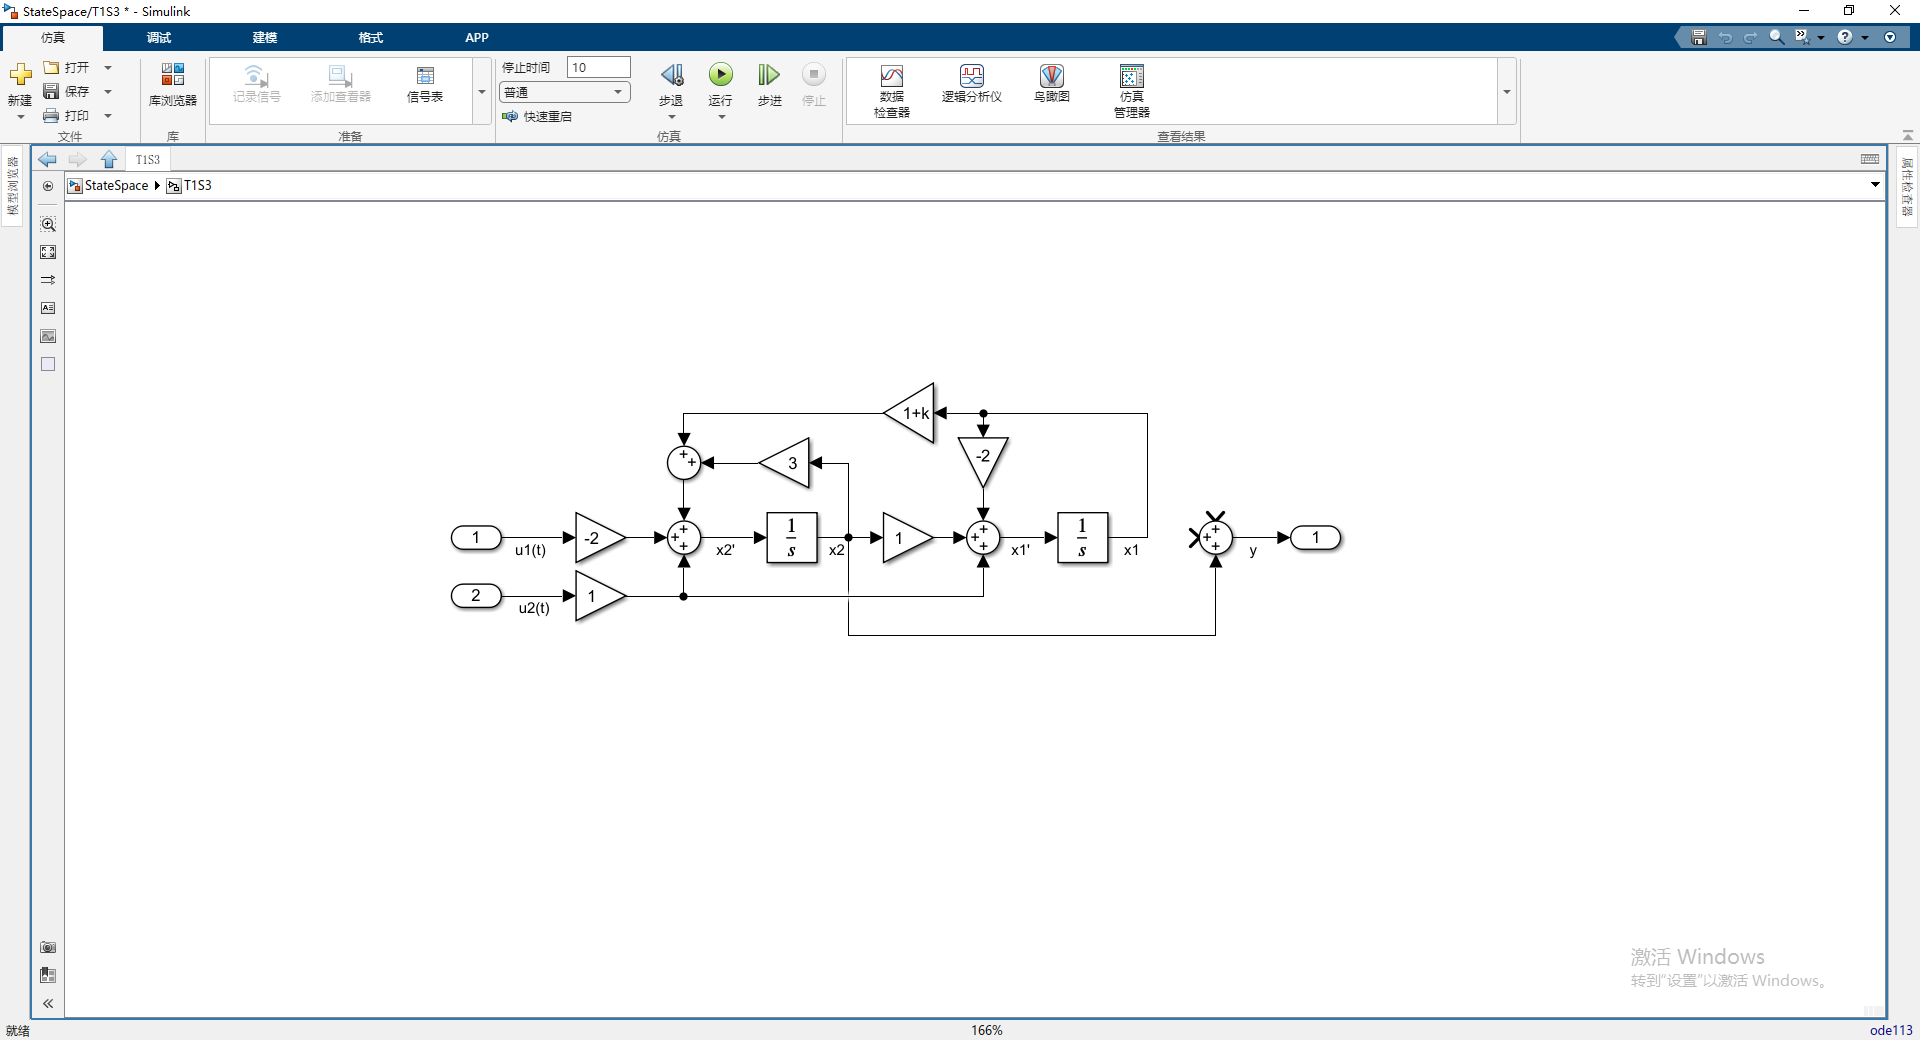
\includegraphics[height = 0.35\textheight]{../screenshots/MT1S3.PNG}
        \caption{System3}
        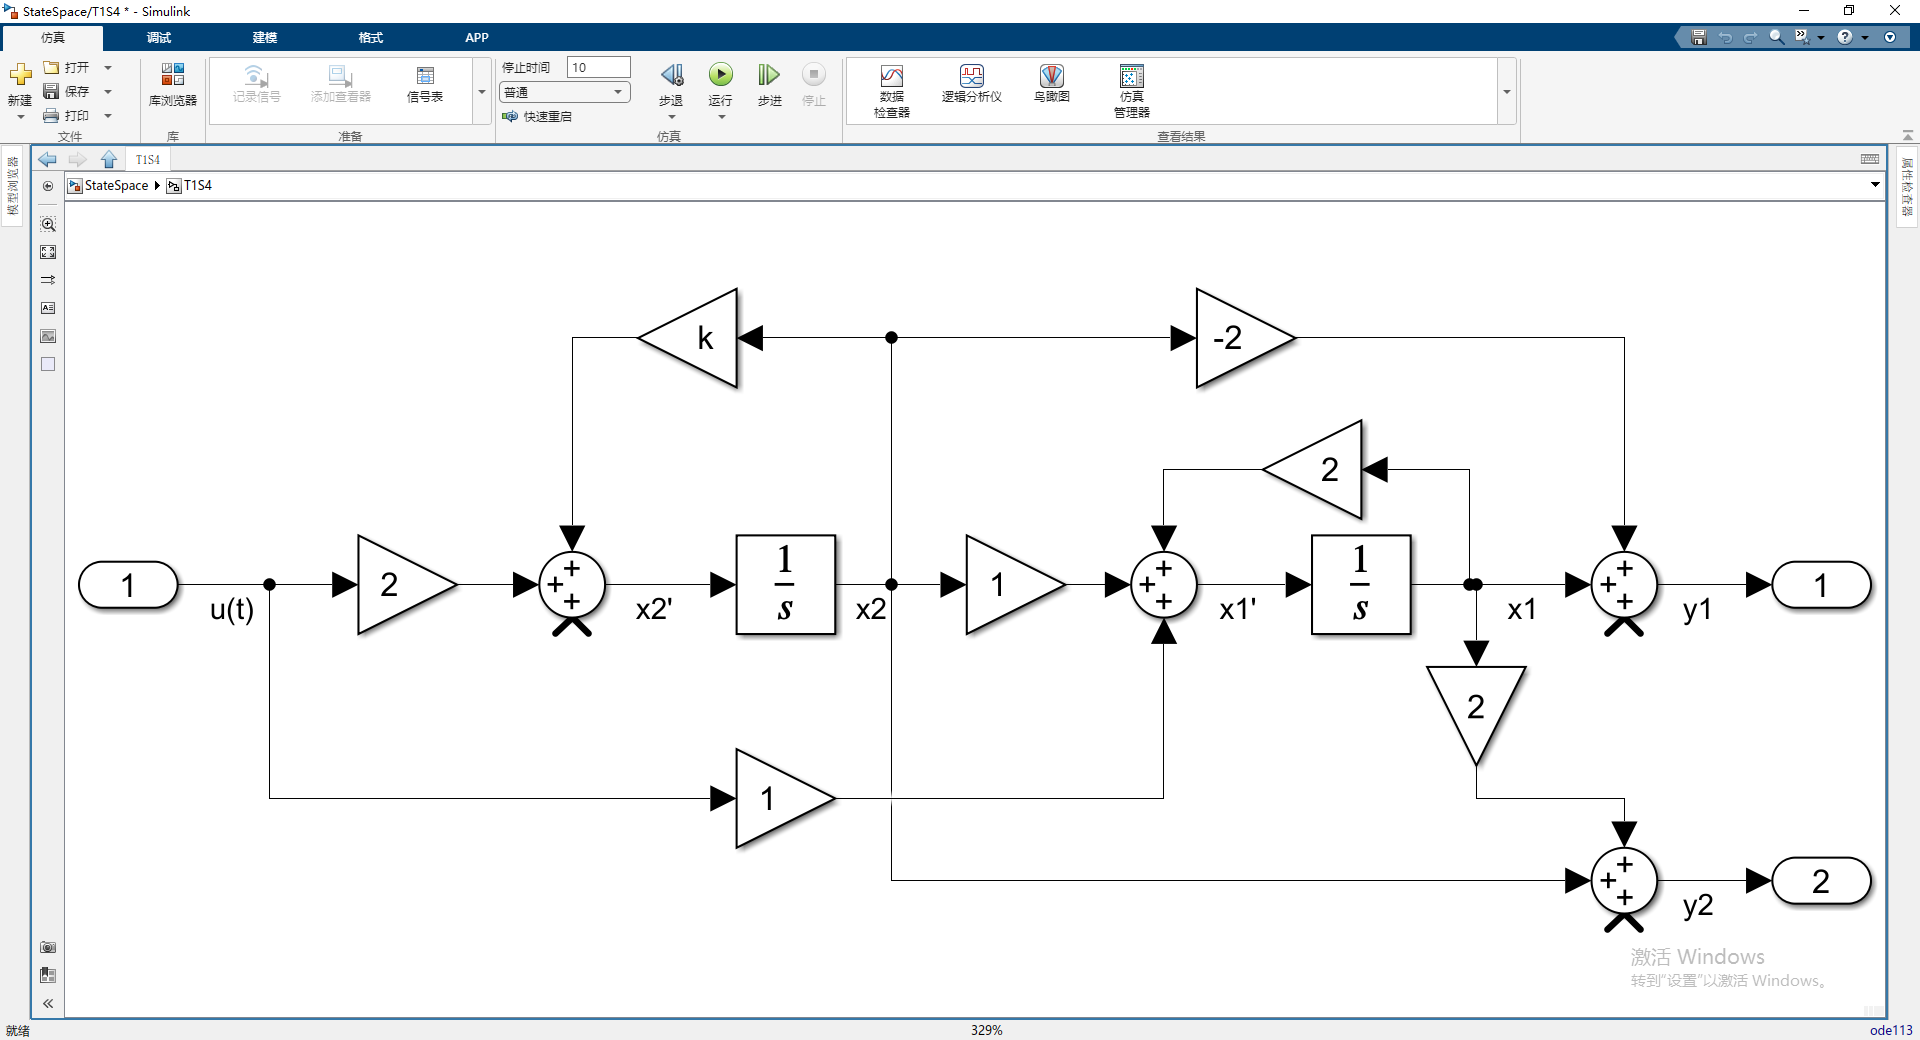
\includegraphics[height = 0.35\textheight]{../screenshots/MT1S4.PNG}
        \caption{System4}
    \end{figure}
    \subsection{Task2}
    \begin{figure}
        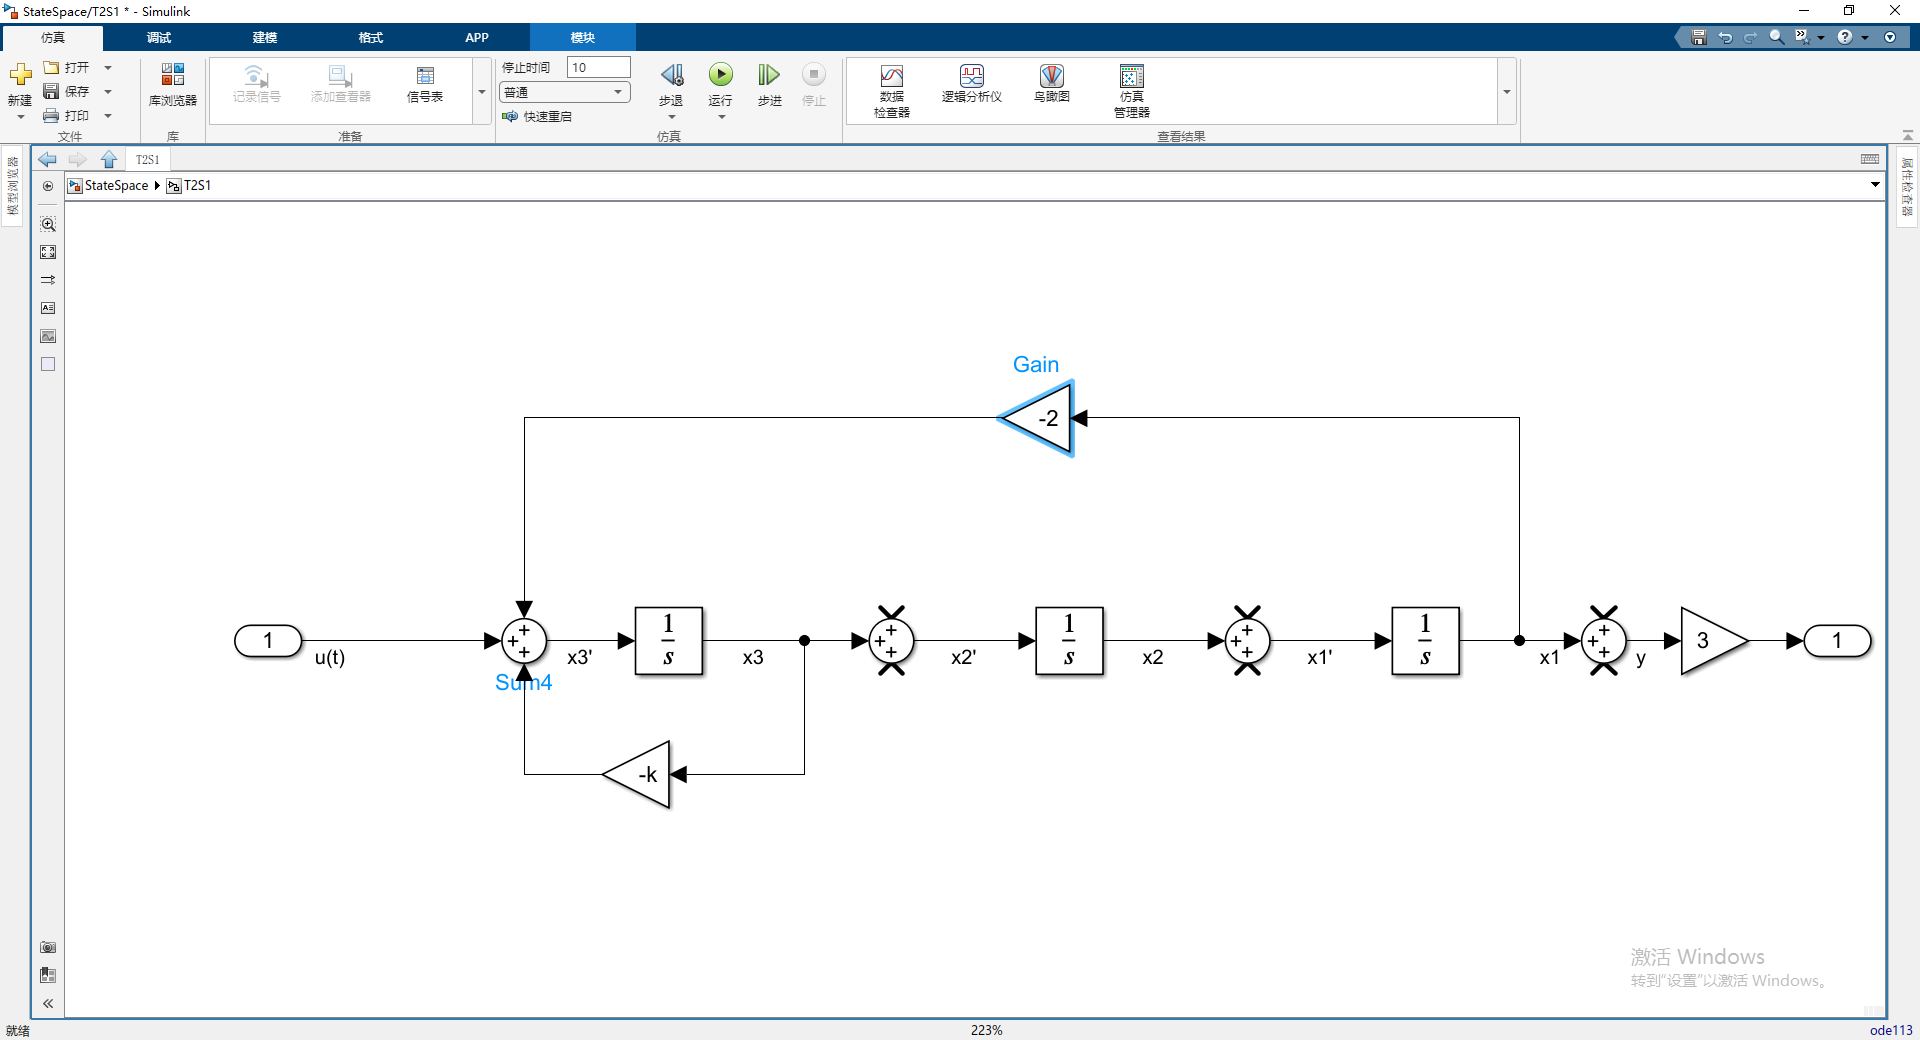
\includegraphics[height = 0.35\textheight]{../screenshots/MT2S1.PNG}
        \caption{System1}
        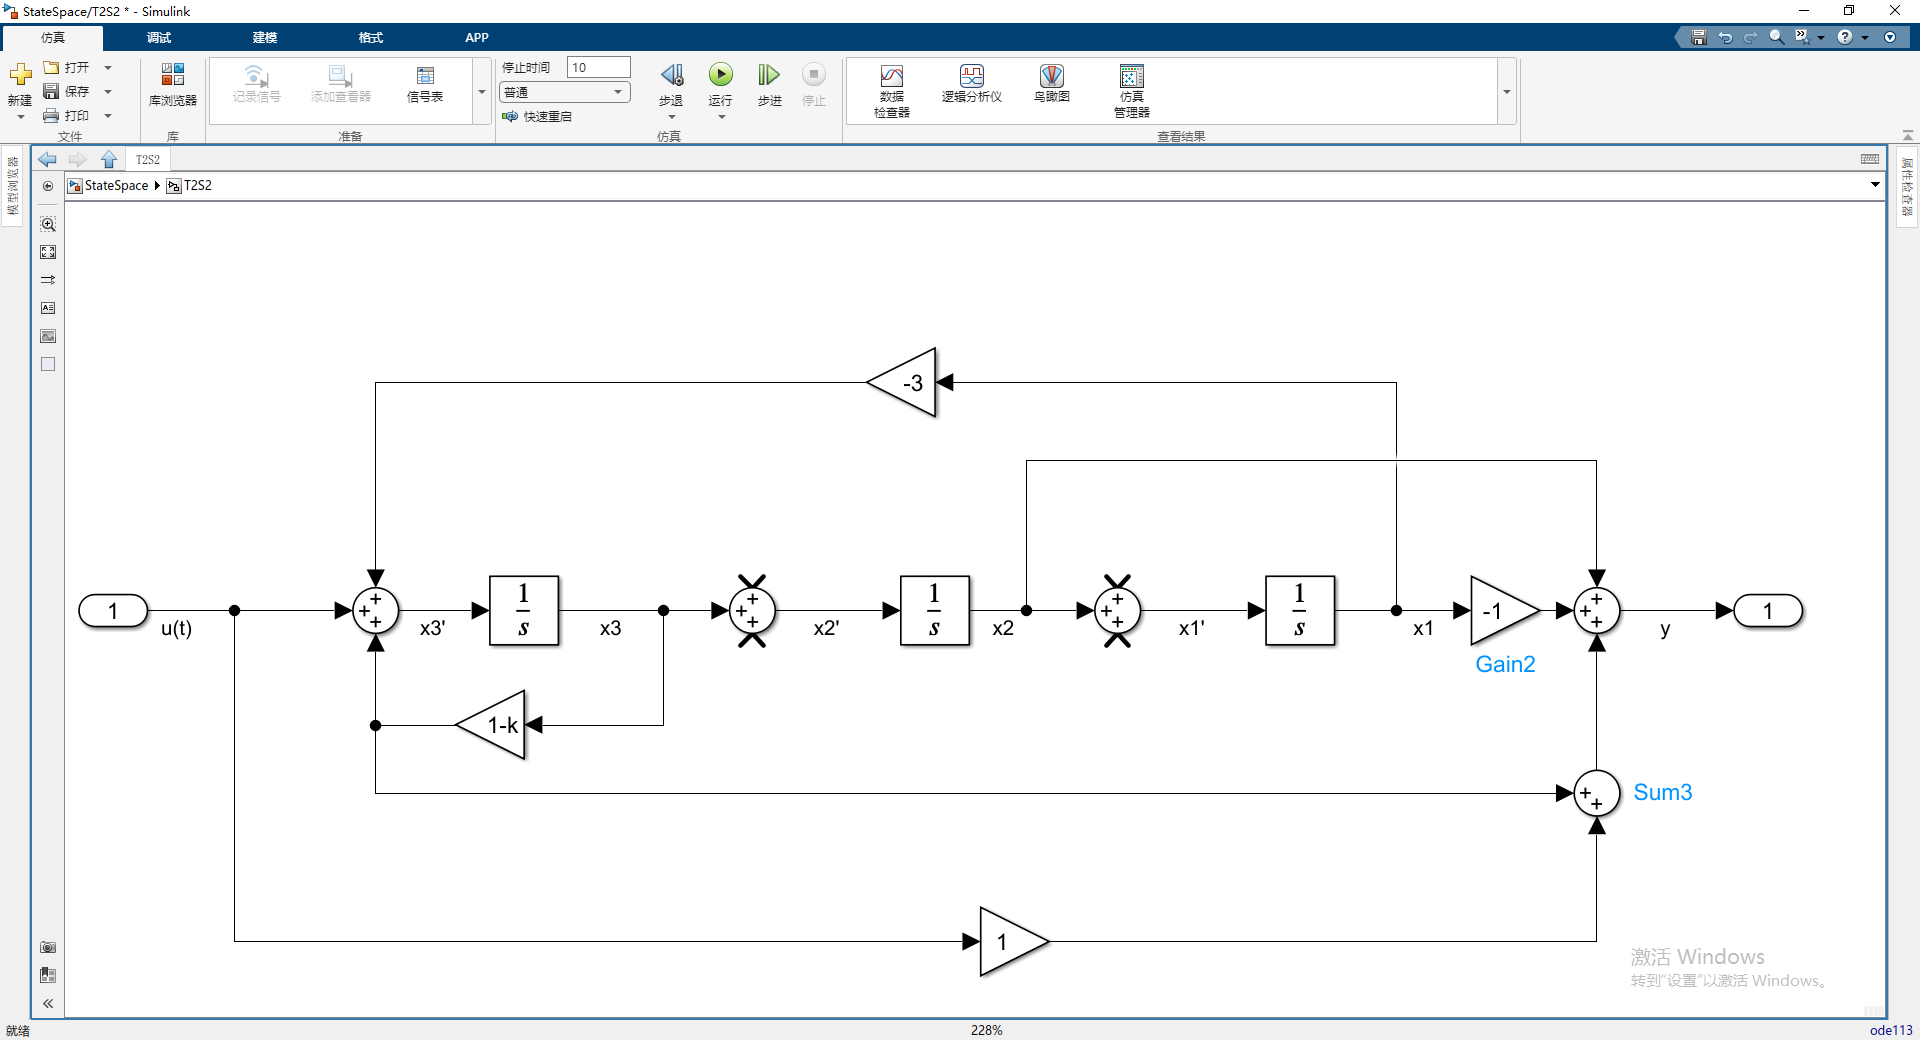
\includegraphics[height = 0.35\textheight]{../screenshots/MT2S2.PNG}
        \caption{System2}
    \end{figure}

    \section{Task1}
    \subsection{Construct the system in MATLAB/Simulink}
    See above section.
    \subsection{Represent the system in the Input-Output form}
    Transfer function model Details:
    \newpage
    \begin{figure}[H]
        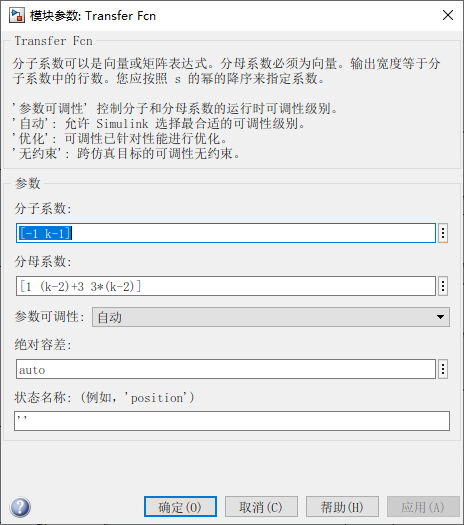
\includegraphics[height = 0.35\textheight]{../screenshots/MT1S1Tran.PNG}
        \caption{System1}
        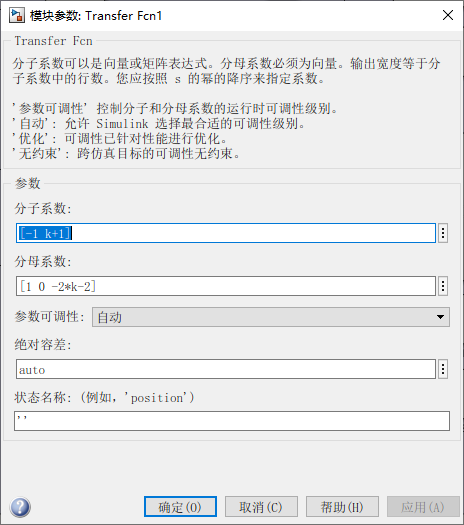
\includegraphics[height = 0.35\textheight]{../screenshots/MT1S2Tran.PNG}
        \caption{System2}
    \end{figure}
    \newpage
    \begin{figure}[H]
        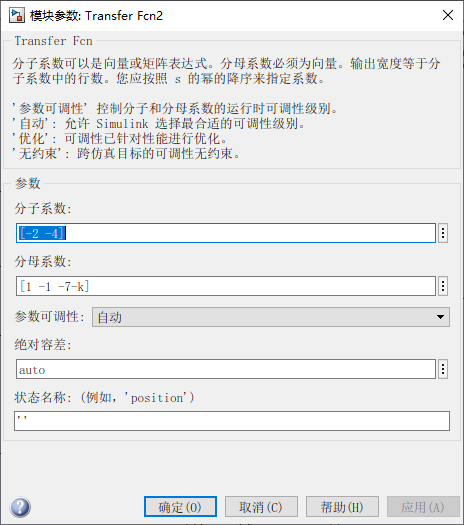
\includegraphics[height = 0.35\textheight]{../screenshots/MT1S3Tran1.PNG}
        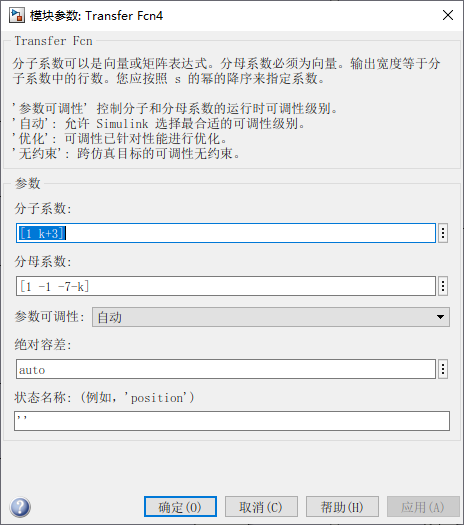
\includegraphics[height = 0.35\textheight]{../screenshots/MT1S3Tran2.PNG}
        \caption{System3}
    \end{figure}
    \begin{figure}[H]
        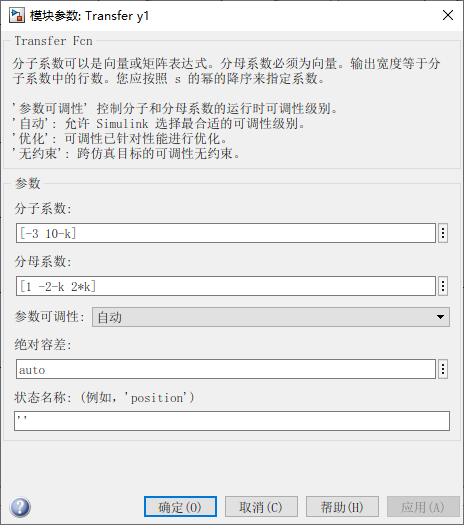
\includegraphics[height = 0.35\textheight]{../screenshots/MT1S4Tran1.PNG}
        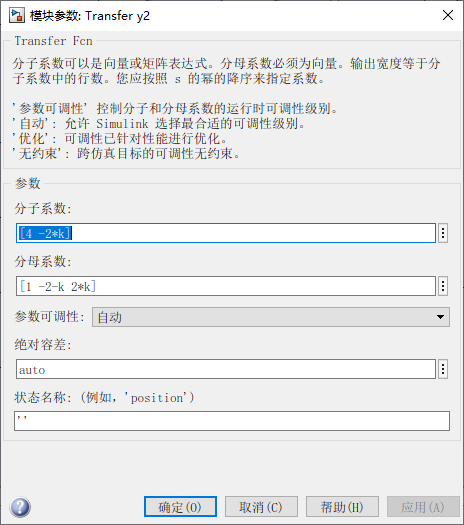
\includegraphics[height = 0.35\textheight]{../screenshots/MT1S4Tran2.PNG}
        \caption{System4}
    \end{figure}

    Calculation by Wolfram Engine:
    \begin{figure}[H]
        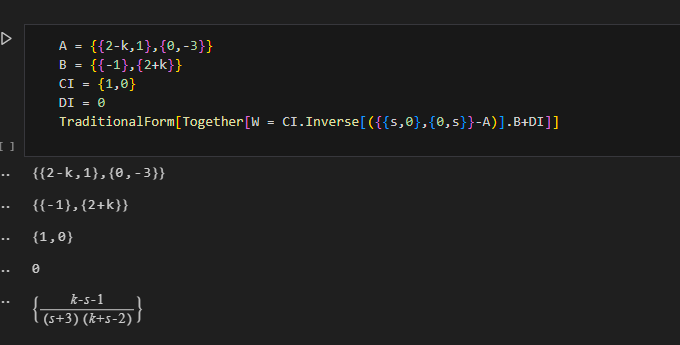
\includegraphics[width = 0.6\linewidth]{../screenshots/WCalcT1S1.PNG}
        \caption{System1}
        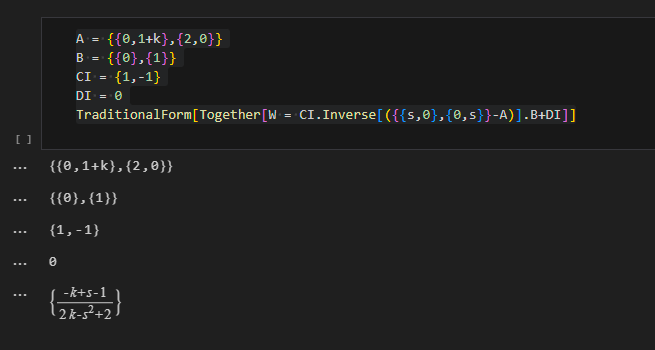
\includegraphics[width = 0.6\linewidth]{../screenshots/WCalcT1S2.PNG}
        \caption{System2}
        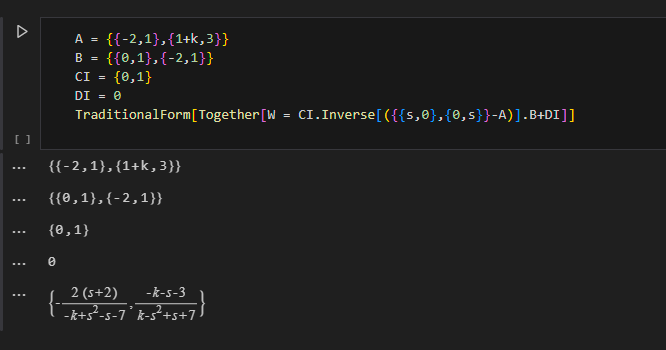
\includegraphics[width = 0.6\linewidth]{../screenshots/WCalcT1S3.PNG}
        \caption{System3}
        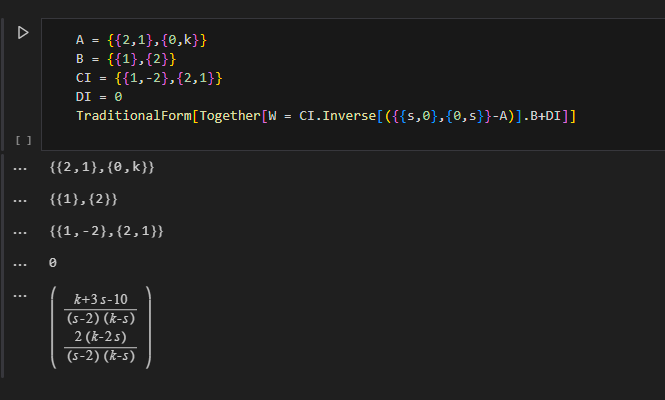
\includegraphics[width = 0.6\linewidth]{../screenshots/WCalcT1S4.PNG}
        \caption{System4}
    \end{figure}
    \newpage
    \subsection{Stablity}
    $$k = 7$$

    For System1:
    $$det(A-\lambda*I) =\begin{vmatrix}
       2-k-\lambda & 1 \\
       0 & -3-\lambda 
    \end{vmatrix} = 0$$
    $$ ->\lambda_1 = -3, \lambda_2 = 2-k $$
    Getting $\lambda_1 = -3, \lambda_2 = -5$ For me.
    \textcolor{red}{So System1 is asymptotically stable in my case, performing \textbf{Node Behavior}.}

    For System2:
    $$det(A-\lambda*I) =\begin{vmatrix}
        0-\lambda & 1+k \\
        2 & 0-\lambda 
     \end{vmatrix} = 0$$
    Getting $\lambda_1 = 4, \lambda_2 = -4$ For me.
    \textcolor{red}{So System2 is not stable in my case, performing \textbf{Saddle Behavior}.}

    For System3:
    $$det(A-\lambda*I) =\begin{vmatrix}
       -2-\lambda & 1 \\
        1+k & 3-\lambda 
     \end{vmatrix} = 0$$
    Getting $\lambda_1 = \frac{1-\sqrt{57}}{2}, \lambda_2 = \frac{1+\sqrt{57}}{2}$ For me.
    \textcolor{red}{So System3 is not stable in my case, performing \textbf{Saddle Behavior}.}

    For System4:
    $$det(A-\lambda*I) =\begin{vmatrix}
        2-\lambda & 1 \\
        0 & k-\lambda 
      \end{vmatrix} = 0$$
    Getting $\lambda_1 = 2, \lambda_2 = 7$ For me.
    \textcolor{red}{So System4 is not stable in my case, performing \textbf{Node Behavior}.}

    \section{Task2}
    \subsection{Represent the system in the canonical State-Space forms}
    System1:
    \subsubsection*{Controlable}
    $A = \begin{bmatrix}
        0&1&0\\
        0&0&1\\
        -2&0&-k
    \end{bmatrix}$

    $B = \begin{bmatrix}
        0\\
        0\\
        1
    \end{bmatrix}$

    $C = \begin{bmatrix}
        3&0&0
    \end{bmatrix}$

    \subsubsection*{Observable}
    $A = \begin{bmatrix}
        -k&1&0\\
        0&0&1\\
        -2&0&0
    \end{bmatrix}$

    $B = \begin{bmatrix}
        0\\
        0\\
        3
    \end{bmatrix}$

    $C = \begin{bmatrix}
        1&0&0
    \end{bmatrix}$

    \newpage
    System2:
    \subsubsection*{Controlable}
    $A = \begin{bmatrix}
        0&1&0\\
        0&0&1\\
        -3&0&k+1
    \end{bmatrix}$

    $B = \begin{bmatrix}
        0\\
        0\\
        1
    \end{bmatrix}$

    $C = \begin{bmatrix}
        2-3&1-0&-k+1
    \end{bmatrix}$

    $D = \textcolor{red}{b_n} = 1$(not $b_0$)

    \subsubsection*{Observable}
    $A = \begin{bmatrix}
        -3&1&0\\
        0&0&1\\
        k+1&0&0
    \end{bmatrix}$

    $B = \begin{bmatrix}
        -k+1\\
        1-0\\
        2-3
    \end{bmatrix}$

    $C = \begin{bmatrix}
        1&0&0
    \end{bmatrix}$

    $D = \textcolor{red}{b_n} = 1$(not $b_0$)

    \subsection{Is system stable for u(t) = 0 ?}
    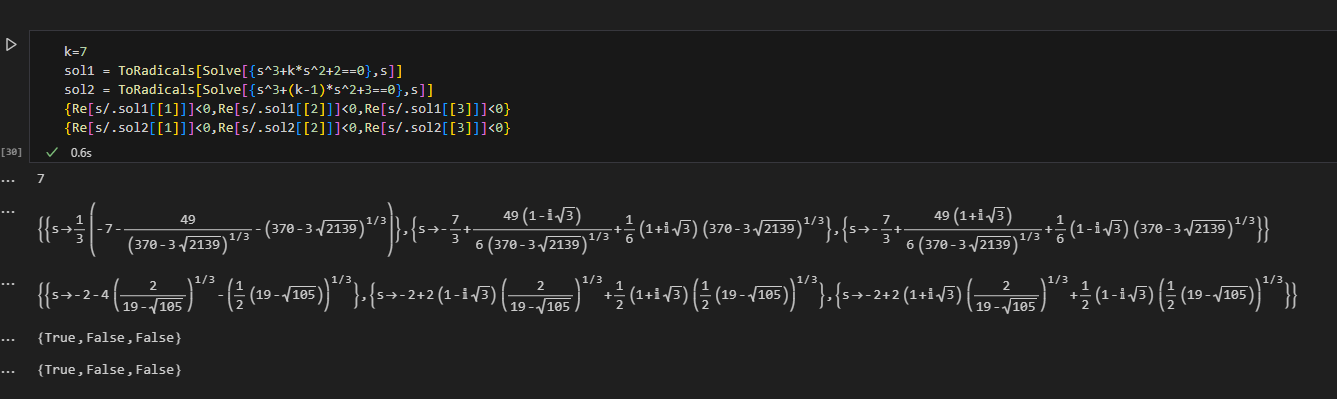
\includegraphics[width = 0.8\linewidth]{../screenshots/SystemStable.PNG}
    
    (Very Complex solve?)
    \textcolor{red}{Not for all $Re(s)<0$,Leading not stable.}
    \subsection{Construct the system in MATLAB/Simulink}
    See section \textbf{Constructing Systems}.

    \section{Figures}
    \subsection{Task1}
    \begin{figure}[H]
        \centering
        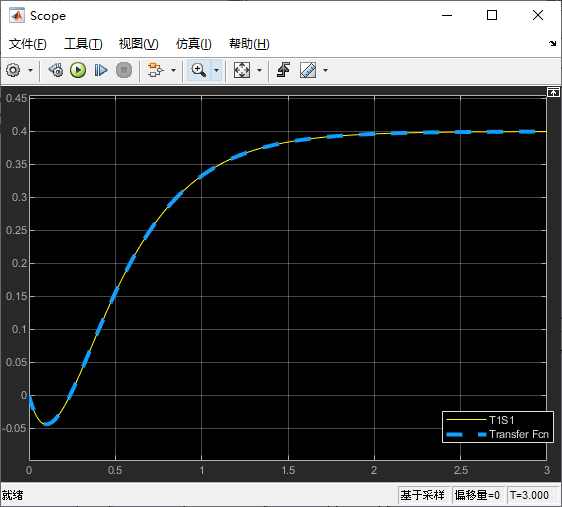
\includegraphics[height = 0.4\textheight]{../screenshots/MT1S1Result.PNG}
        \caption{System1}
        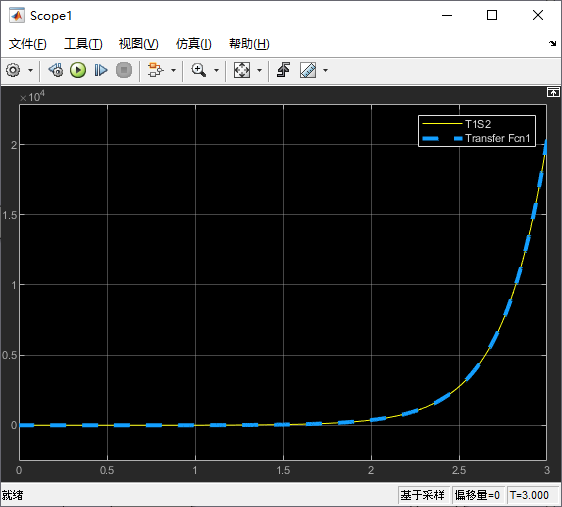
\includegraphics[height = 0.4\textheight]{../screenshots/MT1S2Result.PNG}
        \caption{System2}
    \end{figure}
    \newpage
    \begin{figure}[H]
        \centering
        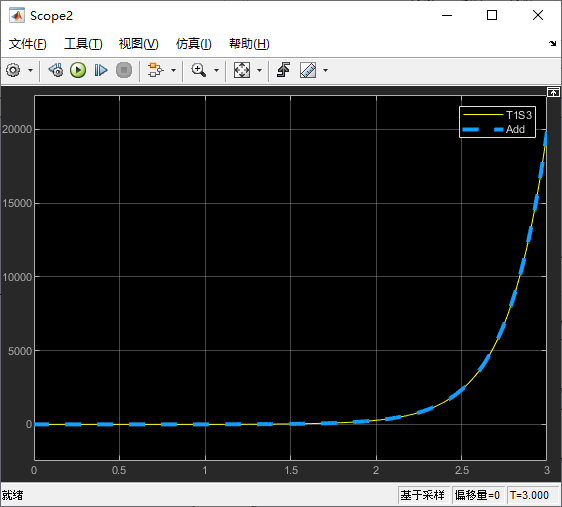
\includegraphics[height = 0.4\textheight]{../screenshots/MT1S3Result.PNG}
        \caption{System3}
        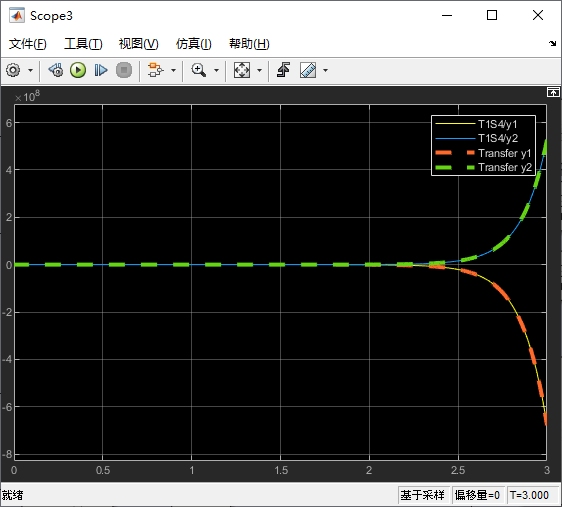
\includegraphics[height = 0.4\textheight]{../screenshots/MT1S4Result.PNG}
        \caption{System4}
    \end{figure}
    \newpage
    \subsection{Task2}
    \begin{figure}[H]
        \centering
        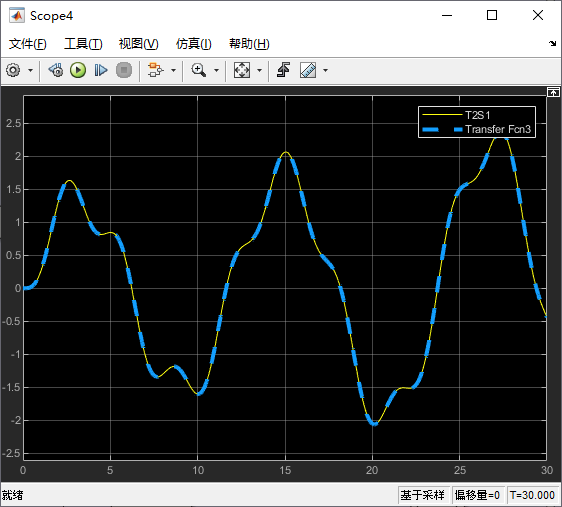
\includegraphics[width = 0.6\linewidth]{../screenshots/MT2S1ResultLT.PNG}
        \caption{System1}
        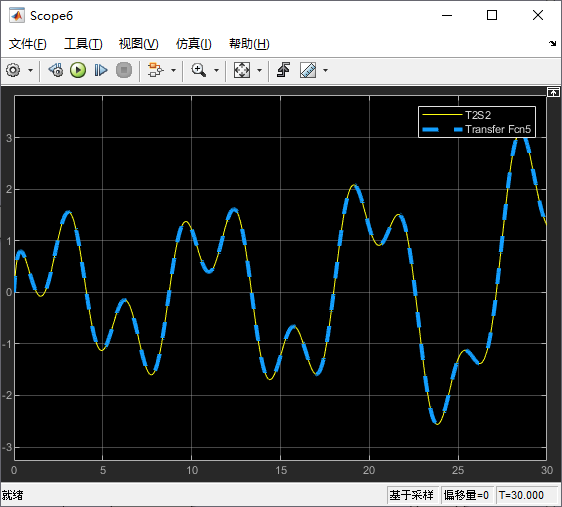
\includegraphics[width = 0.6\linewidth]{../screenshots/MT2S2ResultLT.PNG}
        \caption{System2}
    \end{figure}
\end{document}